\section{Data Collection}

We use the USPTO patent grant full text dataset from January 1995 to December 
2013.  The dataset includes patent number, series code and application number,
type of patent, filing date, title, issue date, inventor information, assignee
name at time of issue, foreign priority information, related US patent
documents, classification information, US and foreign references, attorney,
agent or firm/legal representative, Patent Cooperation Treaty (PCT)
information, abstract, specification, and claims for each patent. We consider
only the following fields from the dataset for our study: patent number, issue
date, inventor name, inventor address, assignee name at time of issue, assignee address, US
references. 


\subsection{Pre-processing}

\begin{itemize}
\item {\em Collection \& Parsing:} We download the patent files from year 2005 to 2013 from the Google's portal for USPTO bulk patent download~\cite{google-uspto}. These files are in various XML formats between v4.0 to v4.4. For the grant data prior to 2005, we use the truncated version from the Harvard DVN database~\cite{harvardDVN}. Then we interpret the structured XML data, read it into python dictionaries and insert the compiled records into our SQLite database. We use the existing tools available from XML parsing and processing written in Python~\cite{funginstitute, fungpaper}. 

\item {\em Disambiguation:} We run the author and organization disambiguation algorithms on this dataset, to cluster the inventors and organizations. Each unique entity is assigned a new internal ID, which we use for our graphs. The information about the disambiguated records is incorporated in the database. 

\item {\em Consolidation and Graph Construction:} 
We consolidate all the datasets together in our SQLite database, and generate the specifics views of data required for constructing the graphs for our further study.
% Finally, we consolidate this data with the pre-processed patent data for years 1975 to 2010 from Harvard Dataverse Network~\cite{}. 
\end{itemize}

Figure~\ref{process} summarizes the data collection, parsing and disambiguation phases we employ in our 
In summary, we extract the following fields from each patent that we parse :

\begin{itemize}
\item {\em Attributes for co-inventor relationship}:
Inventor name, inventor address, assignee name, assignee address, year of patent grant.

\item {\em Attributes for citations}:
Patent ID, name and address of all the inventors and assignees, year of patent grant, all the patents who cites this patent.
\end{itemize}


\subsection{Author \& Organization Disambiguation}

Apart from the primary dataset from USPTO, we use secondary data sets which are necessary for the disambiguation. Specifically, we use the NBER patent database which contains patents granted from 1975-1999, Micropatent, USPTO CASSIS dataset for patent classification, National Geospatial-Intelligence Agency and US Board Geographic Names data sets. The secondary datasets are purely used for disambiguation and is not used for our main evaluation. These data sets are implicitly used for by the disambiguation algorithm available from ~\cite{harvard-dismbi}.

\begin{figure}[H]
		  \centering	
          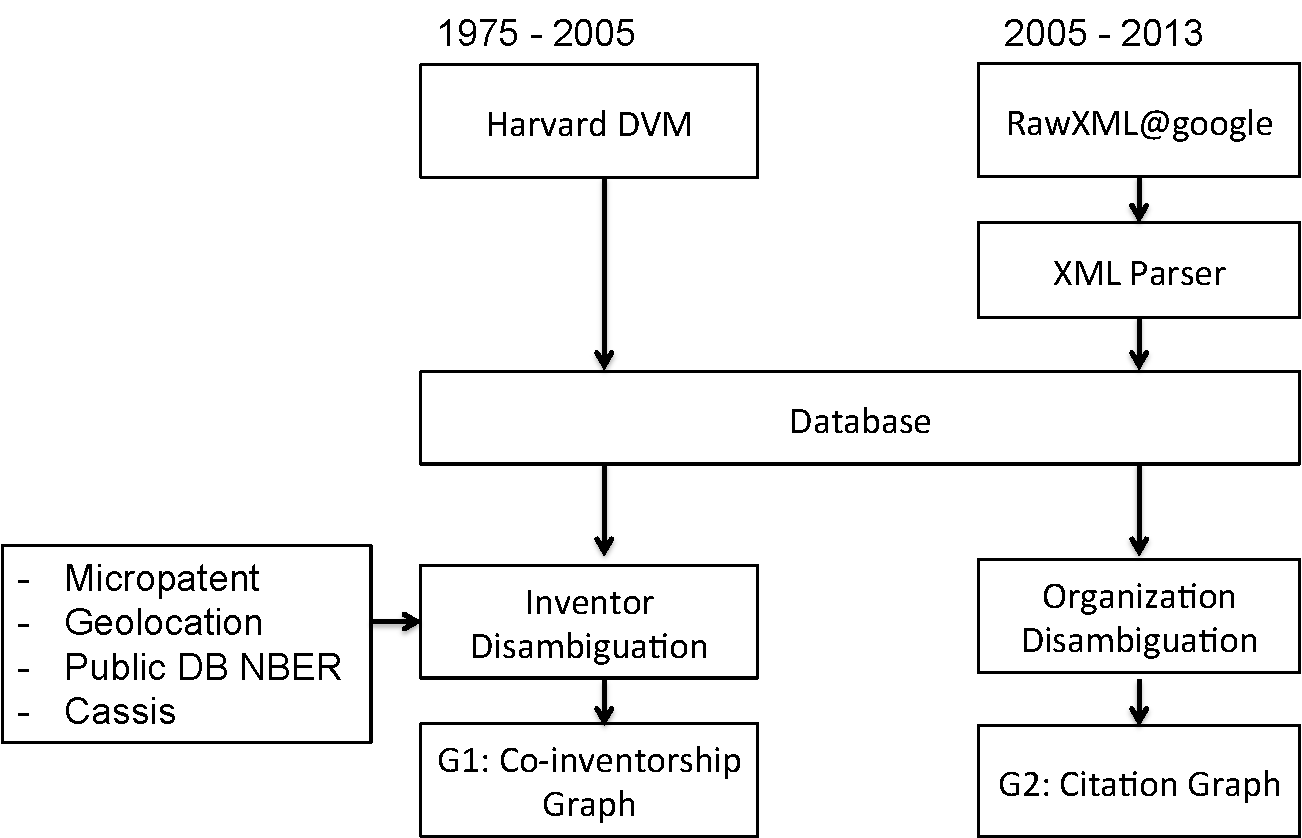
\includegraphics[scale=0.6]{../figures/process.pdf}
          \label{process}
          \caption{Overview of data collection and pre-processing steps to generate the co-inventorship and citation graphs for this study.}
\end{figure}


\subsection{Data Consolidation \& Graph Construction}

We construct two graphs after the disambiguation phase is complete. 
The first graph is for the co-inventor network. 
Each vertex is an inventor, while an edge represents that two inventors have a joint patent. 
We extract this information from our SQLite database, and generate a GraphML file for this network.
Table~\ref{listing} shows an example entry from GraphML for this network.
We report the statistics about the graph size and properties in Section~\cite{sec:eval}.

\begin{table*}[h] 
  \centering
  \begin{tabular}{@{}c@{}} 

  \begin{minipage}{0.25\linewidth}

\begin{lstlisting}[]
<node id="n196819">
  <data key="Loc">BOZEMAN-MT-US</data>
  <data key="Name">BERG, LLOYD</data>
  <data key="id">04292142-1</data>
  <data key="Patents">247</data>
</node>
\end{lstlisting}

  \end{minipage}
  \hspace{0.05\linewidth}
  \begin{minipage}{0.3\linewidth}

\begin{lstlisting}[]
<node id="n471405">
  <data key="Loc">BOZEMAN-MT-US</data>
  <data key="Name">EDISON, THOMAS A</data>
  <data key="id">05147512-2</data>
  <data key="Patents">1</data>
</node>
\end{lstlisting}

  \end{minipage}
  \hspace{0.05\linewidth}
  \begin{minipage}{0.3\linewidth}

\begin{lstlisting}[]
<edge source="n196819" target="n471405">
  <data key="tId">05147512-2</data>
  <data key="hId">04292142-1</data>
  <data key="AppYear">1991</data>
  <data key="Weight">1</data>
</edge>



\end{lstlisting}

  \end{minipage}
  
  \end{tabular}

\label{listing}
\caption{\footnotesize Snippet of entries from GraphXML file. Shows the nodes for Lloyd Berg and Thomas Edison and the corresponding edge between them.}
\end{table*}